
\section{Results/Findings}

%\begin{comment}
\begin{itemize}
    \item Key Results: Present your main findings clearly, using charts, graphs, or diagrams where necessary.
    \item Data Interpretation: Explain the significance of the results in the context of your research objectives.
    \item Unexpected Outcomes: Highlight any results that were unexpected and how they impact your project.
\end{itemize}
%\end{comment}






%#################################################################


\subsection{Key Results}




\begin{comment}
    

\begin{figure}[htbp]
    %\centering
    \raggedright
    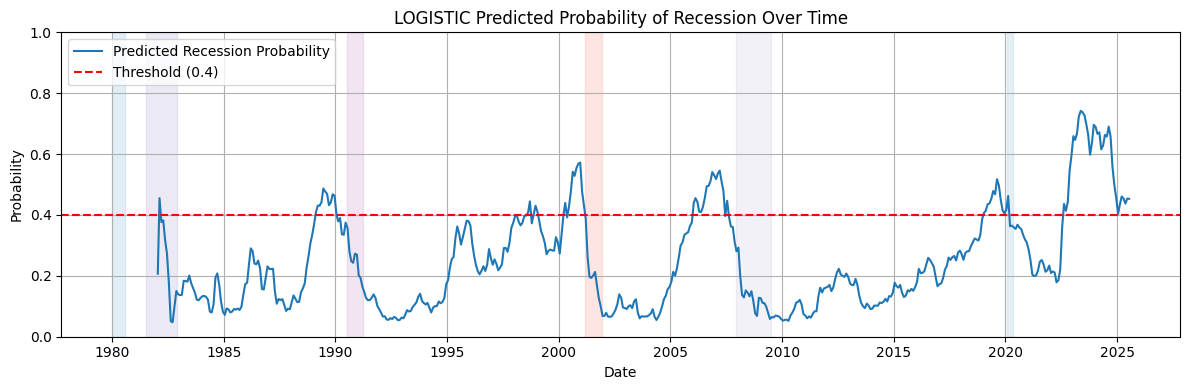
\includegraphics[
        width=\textwidth-24pt, 
        height=\textheight,%-24pt, 
        keepaspectratio
        ]
        {Steps/Plots/LR Predicted Probability of Recession Over Time.png}
    \caption{Predicted Probability of Recession using Logistic Regression . %Inversions (when the spread falls below zero) are often viewed as potential indicators of upcoming economic recessions.
    }
    %\label{fig:yield-spreads}
\end{figure}
\end{comment}

\subsection{Data Interpretation}




\subsection{Unexpected Outcomes}

\begin{comment}
    



let's work on this next

\section{Results/Findings}

\begin{itemize}
    \item Key Results: Present your main findings clearly, using charts, graphs, or diagrams where necessary.
    \item Data Interpretation: Explain the significance of the results in the context of your research objectives.
    \item Unexpected Outcomes: Highlight any results that were unexpected and how they impact your project.
\end{itemize}



{image of class imbalance plot}

\subsection{Key Results}

we would split this into 3 parts

traditional approach, ML, LSTMs


we used SMOTE and Randomundersampler to help out with the class imbalance 
add image of class imbalance

traditional approach; Logistic Regression

Logistic Regression
Metric, No Recession, Recession 
Precision, 0, 0.023681
Recall, 0, 1
F1-Score, 0, 0.046267
auc_pr   ,  0.017529, 0.017529
ap_score ,  0.017913, 0.017913
auc_roc  ,  0.371919, 0.371919

Confusion Matrix
 [[   0 2721]
 [   0   66]]



ML; XGBClassifier, BalancedRandomForestClassifier, EasyEnsembleClassifier

XGBClassifier
Metric, No Recession, Recession 
Precision, 0.964126  , 0.012422 
Recall,    0.474090  , 0.272727 
F1-Score,  0.635625  , 0.023762 
auc_pr  ,  0.016121  , 0.016121
ap_score,  0.016899  , 0.016899
auc_roc ,  0.333261  , 0.333261

Confusion Matrix
 [[1290 1431]
 [  48   18]]


BalancedRandomForestClassifier
Metric, No Recession, Recession 
Precision, 0.962917  , 0.005133  
Recall,    0.572584  , 0.090909  
F1-Score,  0.718138  , 0.009717  
auc_pr  ,  0.014566  , 0.014566
ap_score,  0.017458  , 0.017458
auc_roc ,  0.279317  , 0.279317


Confusion Matrix
 [[1558 1163]
 [  60    6]]



EasyEnsembleClassifier
Metric, No Recession, Recession 
Precision, 0.000000  , 0.023681  
Recall,    0.000000  , 1.000000  
F1-Score,  0.000000  , 0.046267  
auc_pr  ,  0.014456  , 0.014456
ap_score,  0.019808  , 0.019808
auc_roc ,  0.263066  , 0.263066


Confusion Matrix
 [[   0 2721]
 [   0   66]]

\end{comment}

 Here